\documentclass[tikz]{standalone}
\usepackage{pgfplots}
\usepackage{xcolor}
\pgfplotsset{compat=1.18}
\definecolor{planecolor}{HTML}{674ea7}
\definecolor{pointcolor}{HTML}{3c78d8}

\begin{document}
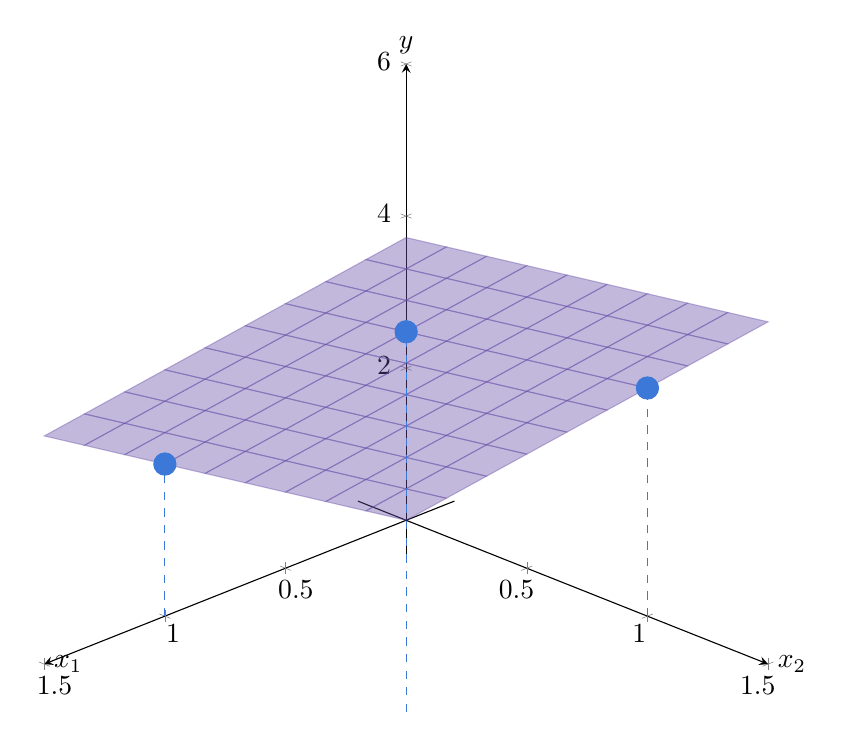
\begin{tikzpicture}
  \begin{axis}[
    view={135}{25},
    xlabel={\(x_1\)},
    ylabel={\(x_2\)},
    zlabel={\(y\)},
    xmin=-0.2, xmax=1.5,
    ymin=-0.2, ymax=1.5,
    zmin=-0.5, zmax=6,
    xtick={0,0.5,1,1.5},
    ytick={0,0.5,1,1.5},
    ztick={0,2,4,6},
    grid=major,
    width=12cm,
    height=12cm,
    axis lines=center,
    xlabel style={anchor=west},
    ylabel style={anchor=west},
    zlabel style={anchor=south},
  ]
    % Best fit plane: y = 2*x1 + 3*x2
    \addplot3[
      surf,
      opacity=0.4,
      color=planecolor,
      faceted color=planecolor,
      samples=10,
      domain=0:1.5,
      y domain=0:1.5,
    ] {2*x + 3*y};

    % Data points: (1,0,2), (0,1,3), (1,1,5)
    \addplot3[
      only marks,
      mark=*,
      mark size=4pt,
      color=pointcolor,
    ] coordinates {
      (1, 0, 2)
      (0, 1, 3)
      (1, 1, 5)
    };

    % Vertical lines from points to plane (to show fit)
    \addplot3[dashed, color=pointcolor, thin] coordinates {(1, 0, 0) (1, 0, 2)};
    \addplot3[dashed, color=pointcolor, thin] coordinates {(0, 1, 0) (0, 1, 3)};
    \addplot3[dashed, color=pointcolor, thin] coordinates {(1, 1, 0) (1, 1, 5)};
  \end{axis}
\end{tikzpicture}
\end{document}
